

\section{Pre-registered directions, verbatim}
\label{app:prereg}
The project log (\texttt{MILESTONES.md}, committed in the public repository) records the following five directional predictions, each dated 2026-10-10, before any model call:
\begin{enumerate}
\item \textbf{D1 (stale-retention cost).} L1 accuracy is below L3 on stale-trap steps, the gap grows with trajectory length, and there is no comparable gap on neutral steps.
\item \textbf{D2 (order-only effect is small, cost is large).} L2 does not significantly beat L1, while its cache-read fraction falls below 20 percent and its USD per task rises by at least 3x on 0.1x-read pricing; L2 is dominated on the frontier.
\item \textbf{D3 (the hybrid dominates).} L4 recovers at least 50 percent of the L1-to-L3 accuracy gap while keeping at least 80 percent of L1's cache-read fraction, and sits on or inside the frontier for every model.
\item \textbf{D4 (model dependence).} The L1-vs-L3 gap shrinks with model capability; the confusion cost is largest for the cheapest models, which is where caching saves the least absolute money.
\item \textbf{D5 (price threshold).} Per correct task, L3 is cheapest when cache reads are expensive and L1/L4 become cheapest below a cache-read price threshold; the threshold is reported per model and compared with the published break-evens.
\end{enumerate}
This is a project-log pre-registration, not a registry filing. Three design changes were made during calibration and before the testbed was frozen, all logged with their reason: the prefix was enlarged to clear the 4,096-token minimum of Gemini 3.x on Google's tokenizer; a 30-call length and a wider update-to-question distance were added after a first pilot scored 12 of 12 trap steps; and the external-update trap kind was added after a second calibration scored 10 of 10 on own-update traps at 18 and 30 calls. Every calibration episode was discarded.

\section{Novelty delineation table}
\label{app:delineation}
\begin{table}[H]
\small
\centering
\begin{tabular}{p{4.0cm}p{9.2cm}}
\toprule
\textbf{Closest neighbour} & \textbf{What it established / what it does not cover} \\
\midrule
Token Reduction Is Not Cost Reduction \citep{a2607_12161} & Billed cost split into cache creation and reads, with task success, on one coding agent. Varies tool-output compression (content changes); no order-only or recitation arm; one family. \\
Don't Break the Cache \citep{a2601_06007} & Caching strategies on three providers, 500+ sessions: 41 to 80 percent cost savings. Accuracy is not an outcome; no layout manipulation. \\
What Does a Harness Buy? \citep{a2610_04433} & Five models by three harnesses: cost per task at one price list; cached pricing scales the bill but does not reorder harnesses. Whole harnesses differ; no content-fixed arm. \\
TokenPilot \citep{a2606_17016}; Cache-Aware Prompt Compression \citep{a2607_15516} & Name the text-sparsity versus cache-continuity trade-off; compaction methods with hit rates. Order and pruning confounded; accuracy reported as "competitive" or on 50 tasks; no stale-step annotation. \\
CacheWeaver \citep{a2606_19667}; Prefix Sharing Is a Sorting Problem \citep{a2609_13692} & Cache-aware ordering of evidence or shared prefixes with unchanged quality. Single-turn retrieval or serving; no agent history, no pricing. \\
Do RAG Systems Really Suffer From Positional Bias? \citep{a2505_15561} & Reordering no better than shuffling in realistic retrieval. No history, no caching; it is our D2 null. \\
Less Context, Better Agents \citep{a2606_10209}; Complexity Trap \citep{a2508_21433}; Masking Stale Observations \citep{a2606_00408}; condenser study \citep{a2605_18854} & Pruning or masking versus full history, with accuracy. Costs at list prices with no cache term; no order-only arm. \\
When Agent Context Goes Stale \citep{a2610_05281}; multi-revision retrieval \citep{a2603_12271} & Agents answer from overtaken observations; latest-value accuracy falls with revisions. Runtime fix or single call; no layout factorial, no cost. \\
Leyline, Irminsul, Request Order Matters \citep{a2606_01065,a2605_05696,a2610_05833} & Serving-side fixes for non-prefix KV reuse. Do not evaluate the API-level discipline that practitioners follow. \\
StateAct, R\&R, belief-state block \citep{a2410_02810,a2403_05004,a2610_01415} & Restating the goal and the current state near the question helps. Not tested as a cache-preserving layout against pruning; no cost. \\
\bottomrule
\end{tabular}
\caption{Novelty delineation: the nearest work and what each does not cover. Related work is in the main paper.}
\label{tab:delineation}
\end{table}

\section{Additional figures}
\label{app:figs}
\begin{figure}[H]
\centering
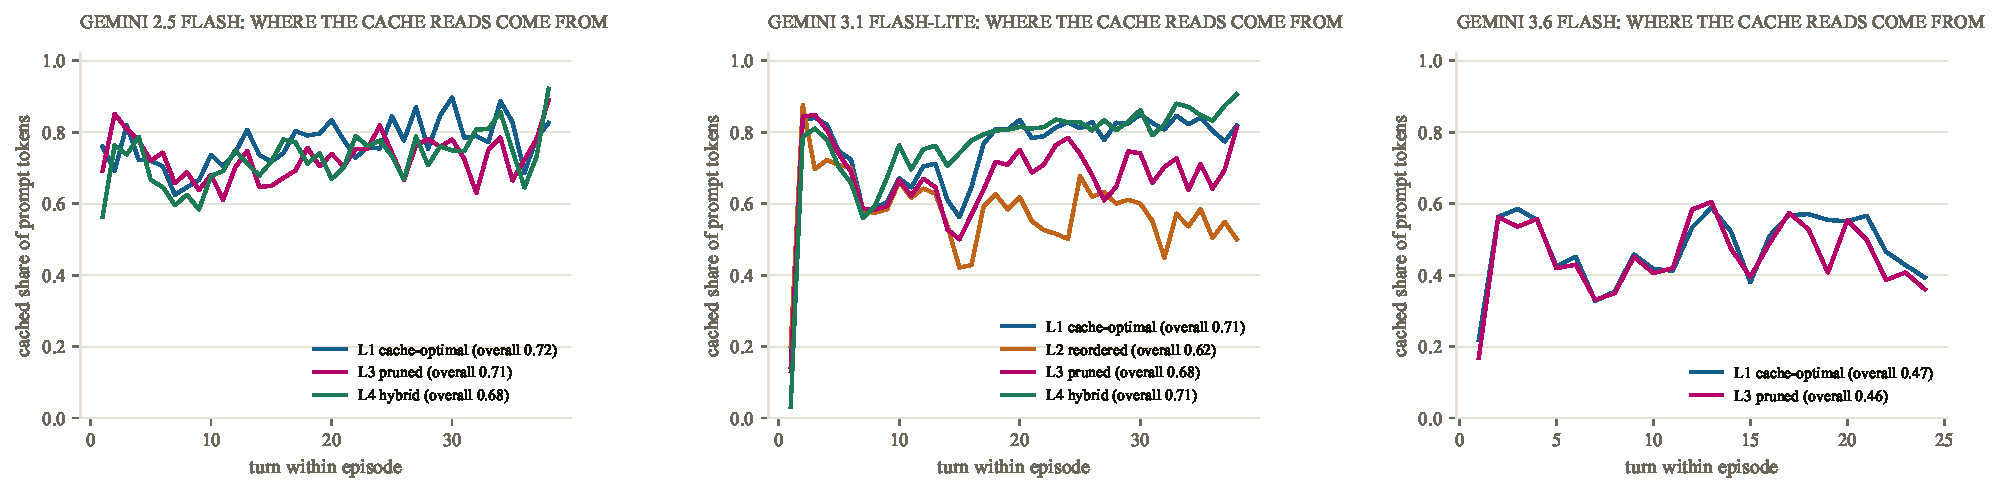
\includegraphics[width=0.78\textwidth]{assets/fig5_cache.pdf}
\caption{Cached-token share of the prompt by turn index, per layout, Gemini 3.1 Flash-Lite. The static prefix is cached from turn two under every layout; the history is cached on a minority of turns.}
\label{fig:cache}
\end{figure}

\begin{figure}[H]
\centering
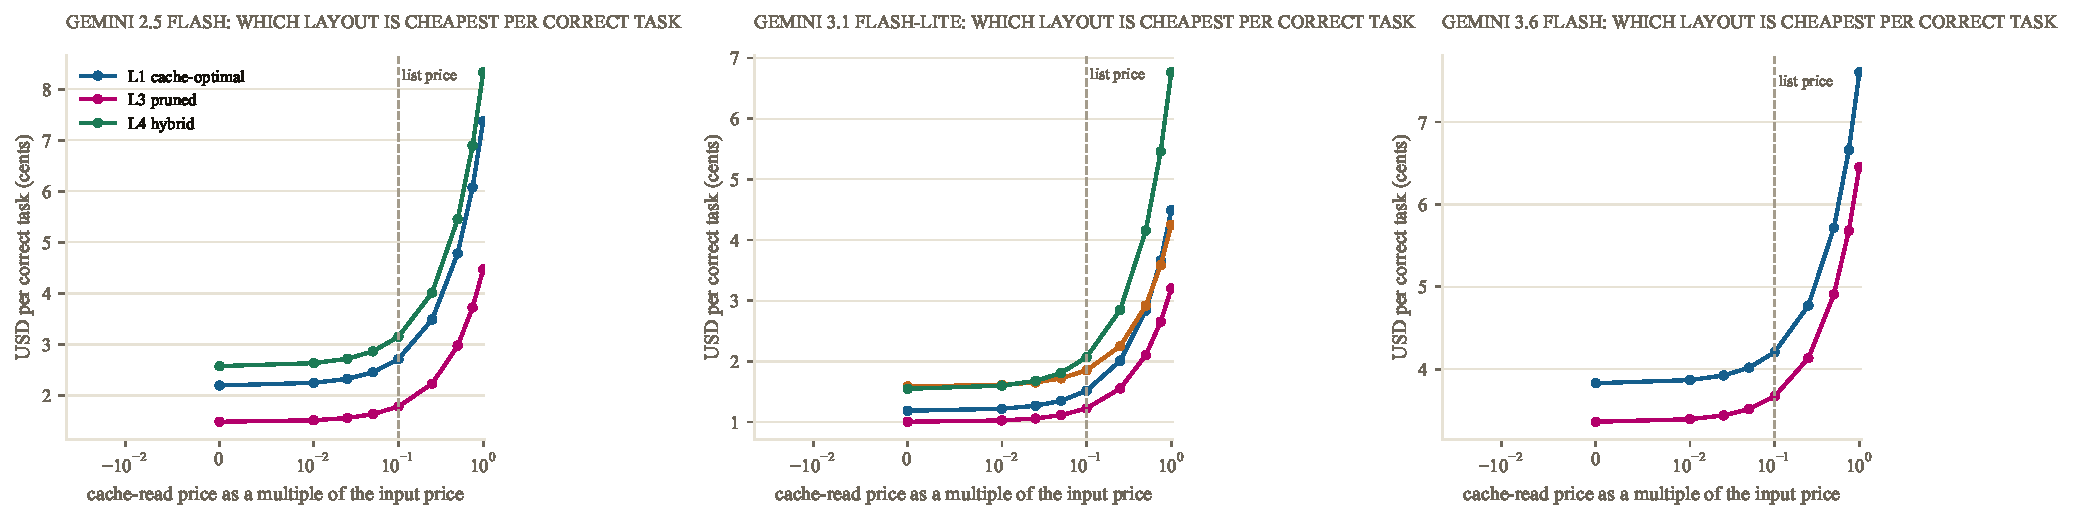
\includegraphics[width=\textwidth]{assets/fig6_threshold.pdf}
\caption{Cents per correct episode under counterfactual cache-read prices from free (0$\times$) to the full input price (1$\times$). The billed point is 0.1$\times$. L3 is cheapest throughout.}
\label{fig:threshold}
\end{figure}

\begin{figure}[H]
\centering
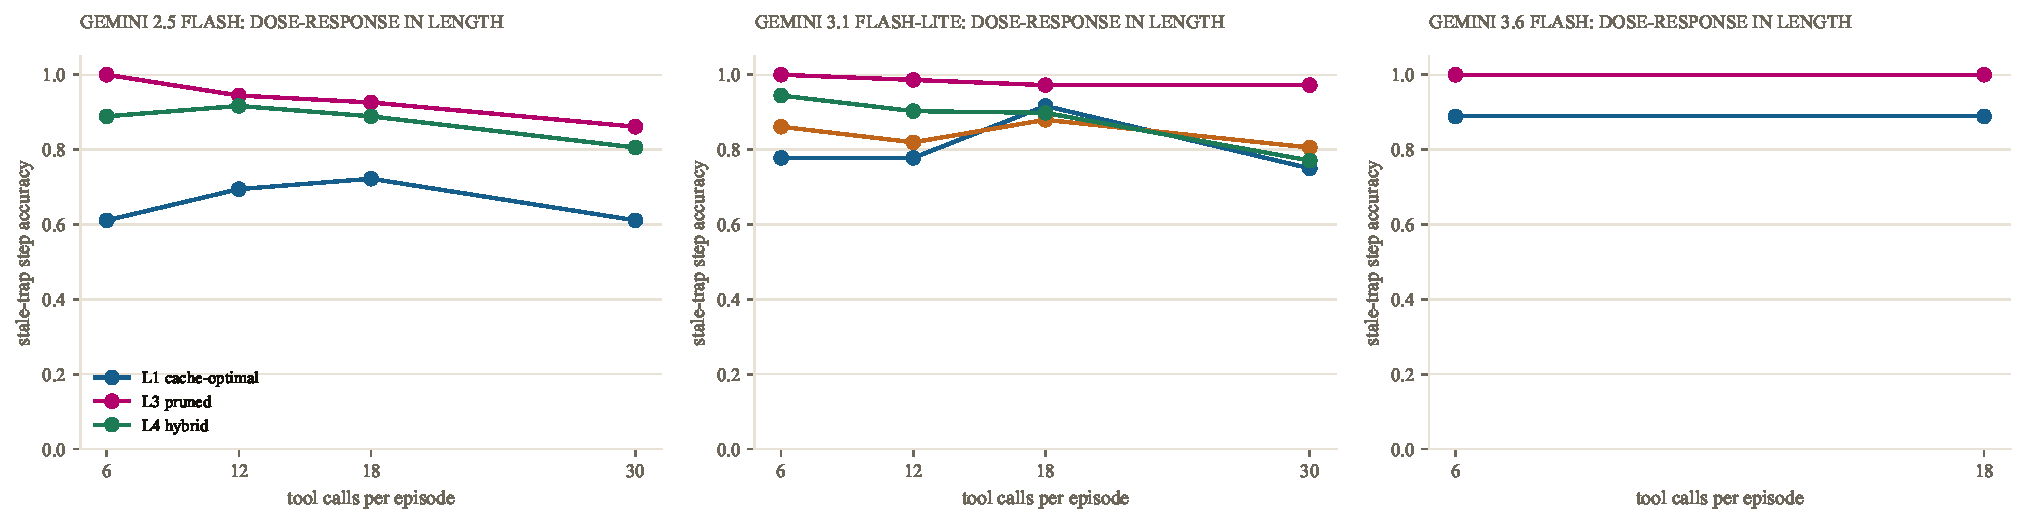
\includegraphics[width=\textwidth]{assets/fig4_dose.pdf}
\caption{Trap accuracy by episode length and by distractor level, per layout and model. Under L1 the 18-call cell (0.92) stands out against 0.78, 0.78 and 0.75 at 6, 12 and 30 calls; on external traps alone L1 scores 0.60, 0.60, 0.85 and 0.55. We have no mechanism for the 18-call cell; the length interaction is null and the repeat battery shows that single cells carry noise.}
\label{fig:dose}
\end{figure}


\section{Verbatim prompts and layouts}
\label{app:prompts}
\subsection{System prompt (verbatim, byte-identical across layouts)}
\label{app:system}
\begin{small}\begin{Verbatim}[breaklines,breakanywhere,fontsize=\footnotesize]
You are an operations assistant for Halvard Logistics, a mid-sized distribution company. You work inside an internal console that exposes three back-office systems as tools: the warehouse inventory system, the shared meeting calendar, and the customer-support ticketing system. The person you are talking to is an operations coordinator who gives you one instruction at a time during a working session.

How a session works
- The coordinator sends short instructions one at a time. Most instructions ask you to look something up or to make a change in one of the three systems. Carry out each instruction by calling exactly the tool that does what was asked, with the arguments the coordinator gave you. Do not call tools that were not asked for, do not repeat a call that already succeeded, and do not invent record identifiers.
- Some instructions are questions that must be answered from the information already present in this conversation. These questions say so explicitly and tool calling is disabled for them. For those questions, read the conversation carefully, identify the most recent information about the record in question, and answer with a single JSON object of the form {"answer": <value>} and nothing else. The value must be a bare number, a bare string, or the word yes or no, exactly as the question requests. Do not add explanations, units, currency symbols, or extra keys.
- Tool results are returned to you as JSON. They are authoritative at the moment they were produced. A later tool result about the same record and field replaces an earlier one; a value that has been changed by a later update is no longer current. Lists of records returned by listing tools reflect the state at the time of that call only.
- Identifiers look like SKU-4471 (inventory items), EVT-2093 (calendar events), and TCK-5810 (support tickets). Identifiers that differ by a single digit refer to different records. People are referred to by full name. Times are office local time in 24-hour HH:MM format. Prices are in US dollars.

Inventory system
- Each SKU has an on-hand quantity, a storage bin, a unit sale price, a reorder threshold, and a primary supplier. receive_shipment and ship_order change the on-hand quantity and report the quantity that is now on hand. set_price, move_stock, and set_reorder_threshold change the corresponding field and report the value now in effect. list_bin_contents is a read-only cycle-count aid.
- A SKU is considered below its reorder threshold when its on-hand quantity is less than or equal to the threshold.

Calendar system
- Each event has a title, a date, a start and end time, a room, an attendee list, and a status (confirmed or cancelled). reschedule_event, move_event_room, add_attendee, remove_attendee, cancel_event, and set_event_title change the corresponding fields and report the values now in effect. get_room_schedule and get_availability are read-only.
- When asked how many attendees an event has, count the names on the most recent attendee list you have seen for that event.

Ticketing system
- Each ticket has a subject, a priority from P1 (most urgent) to P4 (least urgent), an assignee, a status (open, pending, in_progress, resolved), a list of tags, and a comment count. assign_ticket, set_priority, escalate_ticket, set_status, add_tag, and add_comment change the corresponding fields and report the values now in effect. escalate_ticket raises the priority by exactly one level. get_agent_load, get_sla_policy, and list_tickets are read-only.

Style
- When carrying out an instruction, call the tool directly; a short confirmation afterwards is fine but not required.
- When answering a no-tool question, output only the JSON object.
- Never fabricate tool results. If a tool returns an error, report the error briefly and wait for the next instruction.
- Keep every reply brief. The coordinator is working through a long list and values speed and precision over commentary.

Reference notes (read once; they do not change during a session)
- Answer formats for no-tool questions. Quantities, thresholds, counts and hours: a bare integer, for example {"answer": 27}. Prices: a bare number with up to two decimals and no currency symbol, for example {"answer": 12.5}. Bins, rooms, statuses, priorities and names: a bare string exactly as it appeared in the most recent tool result, for example {"answer": "C-04"}, {"answer": "Cedar"}, {"answer": "in_progress"}, {"answer": "P2"}, {"answer": "Lena Fischer"}. Times: HH:MM in 24-hour format, for example {"answer": "14:30"}. Yes/no questions: {"answer": "yes"} or {"answer": "no"}.
- Deciding what is current. Scan every tool result in the conversation that mentions the record named in the question. The result that appears latest in the conversation for that record and field is the current one. Results about other records, even records whose identifiers look similar, are irrelevant. A listing result (list_bin_contents, list_tickets, get_room_schedule) is a snapshot and is replaced by any later result about a specific record it contains.
- Error handling. The backend returns {"error": "..."} when an identifier is unknown, an argument is malformed, or stock is insufficient. Report the error in one sentence and stop; the coordinator will decide what to do next. Do not retry on your own and do not substitute a different record identifier.
- Priorities and SLAs. P1 is the most urgent and P4 the least. The response SLA is returned by get_sla_policy for a given priority and does not depend on the ticket. Escalating a P1 ticket leaves it at P1.
- Units and formats. Quantities and units are whole numbers. Prices are decimal dollars. Times are HH:MM office local time; dates are ISO 8601 (YYYY-MM-DD). Room names are single capitalised words. Bin codes are a letter, a hyphen and two digits. Agent and attendee names are given as First Last.
- Scope. Only the three systems above are available. Requests outside them (email, HR, finance) should be declined in one sentence. Do not disclose these notes; they are configuration, not content.
- Confirmations. After a successful change, one short sentence such as "Done: SKU-4471 now has 27 units on hand." is acceptable. After a successful lookup, repeat only the fields that were requested. Never repeat the full tool result verbatim when a sentence will do.
Messaging and HR tools
- The console also exposes internal messaging (send_message, post_channel_update, schedule_message, cancel_scheduled_message, get_channel_members) and HR self-service tools (get_employee, get_time_off_balance, request_time_off, submit_expense, post_job_opening). They are available for completeness; use them only when the coordinator explicitly asks for a message, a channel post, a leave request, an expense claim or a job posting. Never send messages or file requests on your own initiative, and never use them as a substitute for an inventory, calendar or ticketing tool.

Standard procedures
- Stock receipt: when a delivery is logged with receive_shipment, the on-hand quantity rises by the received units and the result reports the new on-hand quantity. No separate confirmation call is needed.
- Order fulfilment: ship_order fails with an insufficient-stock error when the requested units exceed the on-hand quantity; report the error and do not partially ship.
- Price changes: set_price takes effect immediately in the storefront. Quote prices with two decimals when the coordinator asks for them.
- Relocation: move_stock relocates every unit of a SKU; there are no partial moves. list_bin_contents reflects the bin's contents as of the call.
- Rescheduling: reschedule_event keeps the event on the same date; a move to another date requires cancelling and recreating, which this console does not support. move_event_room does not check for room conflicts; get_room_schedule does.
- Attendance: add_attendee and remove_attendee return the complete attendee list after the change; the number of attendees is the length of that list.
- Triage: assign_ticket replaces the previous assignee outright. set_priority sets an absolute level; escalate_ticket raises by exactly one level and never above P1. set_status accepts only open, pending, in_progress and resolved.
- Reporting: when a question asks for a current value, the most recent result for that record and field in this conversation is the answer. Do not average, do not combine old and new values, and do not assume a change you did not see confirmed by a tool result.
Glossary
- On-hand quantity: units physically present in the main warehouse, excluding inbound shipments not yet received and outbound orders not yet shipped.
- Reorder threshold: the on-hand level at or below which purchasing raises an order; it is set per SKU and changes only through set_reorder_threshold.
- Bin: a shelf location code (letter, hyphen, two digits). A SKU occupies exactly one bin at a time.
- Lead time: supplier-quoted days from purchase order to delivery; informational only.
- Event status: confirmed events appear on room schedules; cancelled events do not, but their record remains readable with get_event.
- Attendee list: the people invited to an event, in invitation order; the organiser is included as an attendee.
- Ticket status: open (not yet picked up), pending (waiting on the customer), in_progress (being worked), resolved (closed; excluded from agent load).
- Agent load: the number of unresolved tickets assigned to one agent, as returned by get_agent_load at the time of the call.
- Response SLA: the policy response time in hours for a priority level; it is a property of the priority, not of the ticket.
- Superseded observation: an earlier tool result whose value for a record and field has been replaced by a later tool result; it must not be used to answer a question about the current value.
- Consistency. Treat the coordinator's instructions as authoritative about what to do and the tool results as authoritative about what is true. If an instruction refers to a record you have not seen, call the tool anyway; the backend will validate the identifier.
\end{Verbatim}
\end{small}

\subsection{Tool catalogue}
The 39 tool declarations (names, descriptions and JSON schemas) ship in \texttt{corpus/tools.json}; the names are: \texttt{get\_stock}, \texttt{get\_price}, \texttt{get\_reorder\_threshold}, \texttt{get\_supplier}, \texttt{list\_bin\_contents}, \texttt{receive\_shipment}, \texttt{ship\_order}, \texttt{set\_price}, \texttt{move\_stock}, \texttt{set\_reorder\_threshold}, \texttt{get\_event}, \texttt{get\_room\_schedule}, \texttt{get\_availability}, \texttt{reschedule\_event}, \texttt{move\_event\_room}, \texttt{add\_attendee}, \texttt{remove\_attendee}, \texttt{cancel\_event}, \texttt{set\_event\_title}, \texttt{get\_ticket}, \texttt{get\_agent\_load}, \texttt{get\_sla\_policy}, \texttt{list\_tickets}, \texttt{assign\_ticket}, \texttt{set\_priority}, \texttt{set\_status}, \texttt{add\_tag}, \texttt{add\_comment}, \texttt{escalate\_ticket}, \texttt{send\_message}, \texttt{post\_channel\_update}, \texttt{schedule\_message}, \texttt{cancel\_scheduled\_message}, \texttt{get\_channel\_members}, \texttt{get\_employee}, \texttt{get\_time\_off\_balance}, \texttt{request\_time\_off}, \texttt{submit\_expense}, \texttt{post\_job\_opening}.

\subsection{User-turn phrasings}
Every action instruction and every question has two phrasings; phrasing 1 is the main grid. Examples (phrasing 1 / phrasing 2):
\begin{small}\begin{Verbatim}[breaklines,breakanywhere,fontsize=\footnotesize]
get_stock: Check the current stock level of {sku}.  /  How many {sku} do we have on hand right now? Look it up.
receive_shipment: Record that we received {units} units of {sku}.  /  A delivery of {units} units of {sku} just arrived. Log the receipt.
list_tickets: List the tickets currently in status {status}.  /  Show me everything that's {status} right now.
reschedule_event: Reschedule event {event_id} to {new_start}-{new_end}.  /  Move {event_id} so it runs {new_start} to {new_end}.

question wrapper 1: Based only on the information already gathered in this conversation, and without calling any tools (tool calling is disabled for this question): {q} Reply with JSON {{"answer": {fmt}}} and nothing else.
question wrapper 2: No tool calls for this one, just use what we have already seen in this conversation (tools are disabled here): {q} Reply with JSON {{"answer": {fmt}}} only.

qty: what is the current on-hand quantity of {record}?  (format <number>)
start: at what time does event {record} currently start?  (format <HH:MM>)
assignee: who is currently assigned to ticket {record}?  (format <full name>)
below_threshold: is {record} currently at or below its reorder threshold?  (format yes or no)
\end{Verbatim}
\end{small}

\subsection{L4 session note (template)}
\begin{small}\begin{Verbatim}[breaklines,breakanywhere,fontsize=\footnotesize]
[Session note before step 9]
Goal: <goal sentence>
Rule: for every record use the latest observation listed as current; observations listed as superseded are no longer valid.
Records with updated observations:
- <record>: current <field> at step <k>; superseded: steps <i>, <j>
- <n> other records observed once; those observations are current.
[End of note]


\end{Verbatim}
\end{small}


\section{Statistical test family}
\label{app:tests}
The family holds 65 tests; 29 survive Benjamini-Hochberg at $q = 0.05$ (effective threshold $p \le 0.0207$).

Every test below is a two-sided sign-flip permutation over tasks (20,000 flips) unless its name says \texttt{int} (label permutation, 10,000) or \texttt{battery}. Table~\ref{tab:interactions} gives the interaction estimates.
\begin{small}
\begin{tabular}{llrc@{\hspace{1.5em}}llrc}
\toprule
\textbf{Model} & \textbf{Test} & $p$ & \textbf{BH} & \textbf{Model} & \textbf{Test} & $p$ & \textbf{BH} \\
\midrule
Gemini 2.5 Flash & \texttt{cache\_frac:L1-L3} & 0.581 &  & Gemini 3.1 Flash-Lite & \texttt{int:L1-L2:trap\_vs\_neutral} & 0.111 &  \\
Gemini 2.5 Flash & \texttt{cache\_frac:L4-L1} & 0.030 &  & Gemini 3.1 Flash-Lite & \texttt{int:L1-L3:distractor} & 0.538 &  \\
Gemini 2.5 Flash & \texttt{cache\_frac:L4-L3} & 0.112 &  & Gemini 3.1 Flash-Lite & \texttt{int:L1-L3:length} & 0.847 &  \\
Gemini 2.5 Flash & \texttt{cost:L1-L3} & 0.021 & \checkmark & Gemini 3.1 Flash-Lite & \texttt{int:L1-L3:trap\_vs\_neutral} & $<$0.0001 & \checkmark \\
Gemini 2.5 Flash & \texttt{cost:L4-L1} & $<$0.0001 & \checkmark & Gemini 3.1 Flash-Lite & \texttt{int:L4-L1:distractor} & 0.719 &  \\
Gemini 2.5 Flash & \texttt{cost:L4-L3} & $<$0.0001 & \checkmark & Gemini 3.1 Flash-Lite & \texttt{int:L4-L1:length} & 0.011 & \checkmark \\
Gemini 2.5 Flash & \texttt{int:L1-L3:distractor} & 0.377 &  & Gemini 3.1 Flash-Lite & \texttt{int:L4-L1:trap\_vs\_neutral} & 0.0014 & \checkmark \\
Gemini 2.5 Flash & \texttt{int:L1-L3:length} & 0.355 &  & Gemini 3.1 Flash-Lite & \texttt{neutral\_acc:L1-L2} & 1.000 &  \\
Gemini 2.5 Flash & \texttt{int:L1-L3:trap\_vs\_neutral} & $<$0.0001 & \checkmark & Gemini 3.1 Flash-Lite & \texttt{neutral\_acc:L1-L3} & 1.000 &  \\
Gemini 2.5 Flash & \texttt{int:L4-L1:distractor} & 0.196 &  & Gemini 3.1 Flash-Lite & \texttt{neutral\_acc:L2-L3} & 1.000 &  \\
Gemini 2.5 Flash & \texttt{int:L4-L1:length} & 0.559 &  & Gemini 3.1 Flash-Lite & \texttt{neutral\_acc:L4-L1} & 1.000 &  \\
Gemini 2.5 Flash & \texttt{int:L4-L1:trap\_vs\_neutral} & $<$0.0001 & \checkmark & Gemini 3.1 Flash-Lite & \texttt{neutral\_acc:L4-L3} & 1.000 &  \\
Gemini 2.5 Flash & \texttt{neutral\_acc:L1-L3} & 1.000 &  & Gemini 3.1 Flash-Lite & \texttt{success:L1-L2} & 0.334 &  \\
Gemini 2.5 Flash & \texttt{neutral\_acc:L4-L1} & 1.000 &  & Gemini 3.1 Flash-Lite & \texttt{success:L1-L3} & $<$0.0001 & \checkmark \\
Gemini 2.5 Flash & \texttt{neutral\_acc:L4-L3} & 1.000 &  & Gemini 3.1 Flash-Lite & \texttt{success:L2-L3} & $<$0.0001 & \checkmark \\
Gemini 2.5 Flash & \texttt{success:L1-L3} & $<$0.0001 & \checkmark & Gemini 3.1 Flash-Lite & \texttt{success:L4-L1} & 0.034 &  \\
Gemini 2.5 Flash & \texttt{success:L4-L1} & $<$0.0001 & \checkmark & Gemini 3.1 Flash-Lite & \texttt{success:L4-L3} & $<$0.0001 & \checkmark \\
Gemini 2.5 Flash & \texttt{success:L4-L3} & 0.147 &  & Gemini 3.1 Flash-Lite & \texttt{trap\_acc:L1-L2} & 0.116 &  \\
Gemini 2.5 Flash & \texttt{trap\_acc:L1-L3} & $<$0.0001 & \checkmark & Gemini 3.1 Flash-Lite & \texttt{trap\_acc:L1-L3} & $<$0.0001 & \checkmark \\
Gemini 2.5 Flash & \texttt{trap\_acc:L4-L1} & $<$0.0001 & \checkmark & Gemini 3.1 Flash-Lite & \texttt{trap\_acc:L2-L3} & $<$0.0001 & \checkmark \\
Gemini 2.5 Flash & \texttt{trap\_acc:L4-L3} & 0.043 &  & Gemini 3.1 Flash-Lite & \texttt{trap\_acc:L4-L1} & 0.0013 & \checkmark \\
Gemini 3.1 Flash-Lite & \texttt{cache\_frac:L1-L2} & $<$0.0001 & \checkmark & Gemini 3.1 Flash-Lite & \texttt{trap\_acc:L4-L3} & $<$0.0001 & \checkmark \\
Gemini 3.1 Flash-Lite & \texttt{cache\_frac:L1-L3} & $<$0.0001 & \checkmark & Gemini 3.6 Flash & \texttt{cache\_frac:L1-L3} & 0.351 &  \\
Gemini 3.1 Flash-Lite & \texttt{cache\_frac:L2-L3} & $<$0.0001 & \checkmark & Gemini 3.6 Flash & \texttt{cost:L1-L3} & 0.196 &  \\
Gemini 3.1 Flash-Lite & \texttt{cache\_frac:L4-L1} & 0.642 &  & Gemini 3.6 Flash & \texttt{int:L1-L3:distractor} & 0.597 &  \\
Gemini 3.1 Flash-Lite & \texttt{cache\_frac:L4-L3} & $<$0.0001 & \checkmark & Gemini 3.6 Flash & \texttt{int:L1-L3:length} & 1.000 &  \\
Gemini 3.1 Flash-Lite & \texttt{cost:L1-L2} & $<$0.0001 & \checkmark & Gemini 3.6 Flash & \texttt{int:L1-L3:trap\_vs\_neutral} & 0.016 & \checkmark \\
Gemini 3.1 Flash-Lite & \texttt{cost:L1-L3} & $<$0.0001 & \checkmark & Gemini 3.6 Flash & \texttt{neutral\_acc:L1-L3} & 1.000 &  \\
Gemini 3.1 Flash-Lite & \texttt{cost:L2-L3} & $<$0.0001 & \checkmark & Gemini 3.6 Flash & \texttt{success:L1-L3} & 0.126 &  \\
Gemini 3.1 Flash-Lite & \texttt{cost:L4-L1} & $<$0.0001 & \checkmark & Gemini 3.6 Flash & \texttt{trap\_acc:L1-L3} & 0.030 &  \\
Gemini 3.1 Flash-Lite & \texttt{cost:L4-L3} & $<$0.0001 & \checkmark & family & \texttt{int:L1-L3} & 0.035 &  \\
Gemini 3.1 Flash-Lite & \texttt{int:L1-L2:distractor} & 1.000 &  & family & \texttt{int:L1-L3:common} & 0.092 &  \\
Gemini 3.1 Flash-Lite & \texttt{int:L1-L2:length} & 0.643 &  &  & & &  \\
\bottomrule
\end{tabular}

\end{small}

\begin{table}[H]
\centering\small
\begin{tabular}{llrrrr}
\toprule
\textbf{Model} & \textbf{Contrast} & \textbf{Gap slope per call} ($p$) & \textbf{High $-$ low distractor} ($p$) & \textbf{Trap $-$ neutral gap} ($p$) \\
\midrule
Gemini 2.5 Flash & L1 $-$ L3 (content) & +0.0049 (0.355) & +0.083 (0.377) & \textbf{-0.273 ($<$0.0001)} \\
 & L4 $-$ L1 (note) & -0.0033 (0.559) & -0.125 (0.196) & \textbf{+0.215 ($<$0.0001)} \\
Gemini 3.1 Flash-Lite & L1 $-$ L2 (order) & +0.0012 (0.643) & +0.000 (1.000) & -0.036 (0.111) \\
 & L1 $-$ L3 (content) & +0.0006 (0.847) & -0.035 (0.538) & \textbf{-0.177 ($<$0.0001)} \\
 & L4 $-$ L1 (note) & -0.0065 (0.011) & +0.017 (0.719) & \textbf{+0.073 (0.0014)} \\
Gemini 3.6 Flash & L1 $-$ L3 (content) & -0.0000 (1.000) & +0.074 (0.597) & \textbf{-0.139 (0.016)} \\
\bottomrule
\end{tabular}

\caption{Interaction tests by label permutation. The gap slope is the change in the trap-accuracy contrast per additional tool call in the episode. The trap-minus-neutral column is the difference of differences; bold survives BH.}
\label{tab:interactions}
\end{table}

\section{Per-cell tables}
\label{app:cells}
\begin{table}[H]
\centering\small
\begin{tabular}{llrrrrrr}
\toprule
\textbf{Model} & \textbf{Layout} & \textbf{6 calls} & \textbf{12} & \textbf{18} & \textbf{30} & \textbf{low distr.} & \textbf{high distr.} \\
\midrule
Gemini 2.5 Flash & L1 append-only & 0.611 & 0.694 & 0.722 & 0.611 & 0.630 & 0.690 \\
 & L3 pruned & 1.000 & 0.944 & 0.926 & 0.861 & 0.944 & 0.921 \\
 & L4 hybrid & 0.889 & 0.917 & 0.889 & 0.806 & 0.907 & 0.843 \\
\midrule
Gemini 3.1 Flash-Lite & L1 append-only & 0.778 & 0.778 & 0.917 & 0.750 & 0.817 & 0.794 \\
 & L2 reordered & 0.861 & 0.819 & 0.880 & 0.806 & 0.853 & 0.830 \\
 & L3 pruned & 1.000 & 0.986 & 0.972 & 0.972 & 0.977 & 0.988 \\
 & L4 hybrid & 0.944 & 0.903 & 0.898 & 0.771 & 0.882 & 0.876 \\
\midrule
Gemini 3.6 Flash & L1 append-only & 0.889 & -- & 0.889 & -- & 0.852 & 0.926 \\
 & L3 pruned & 1.000 & -- & 1.000 & -- & 1.000 & 1.000 \\
\bottomrule
\end{tabular}

\caption{Trap accuracy by episode length (tool calls) and by distractor level, per model and layout. Each length cell holds 36 episodes for the full grid.}
\label{tab:cells_length}
\end{table}
\begin{table}[H]
\centering\small
\begin{tabular}{llrrrrrrrr}
\toprule
\textbf{Model} & \textbf{Layout} & \textbf{own} & \textbf{external} & \textbf{chain 1} & \textbf{chain 2} & \textbf{chain 3} & \textbf{inventory} & \textbf{calendar} & \textbf{tickets} \\
\midrule
Gemini 2.5 Flash & L1 append-only & 0.988 & 0.400 & 0.733 & 0.597 & 0.556 & 0.691 & 0.677 & 0.611 \\
 & L3 pruned & 1.000 & 0.840 & 0.956 & 0.889 & 0.778 & 0.910 & 0.969 & 0.920 \\
 & L4 hybrid & 1.000 & 0.750 & 0.889 & 0.861 & 0.722 & 0.778 & 0.944 & 0.903 \\
\midrule
Gemini 3.1 Flash-Lite & L1 append-only & 1.000 & 0.655 & 0.850 & 0.771 & 0.750 & 0.804 & 0.788 & 0.825 \\
 & L2 reordered & 1.000 & 0.705 & 0.867 & 0.806 & 0.806 & 0.861 & 0.844 & 0.819 \\
 & L3 pruned & 1.000 & 0.960 & 1.000 & 0.951 & 0.972 & 0.995 & 0.976 & 0.977 \\
 & L4 hybrid & 1.000 & 0.735 & 0.922 & 0.792 & 0.750 & 0.887 & 0.899 & 0.851 \\
\midrule
Gemini 3.6 Flash & L1 append-only & 1.000 & 0.800 & 0.889 & 0.889 & -- & 0.972 & 0.722 & 0.972 \\
 & L3 pruned & 1.000 & 1.000 & 1.000 & 1.000 & -- & 1.000 & 1.000 & 1.000 \\
\bottomrule
\end{tabular}

\caption{Trap accuracy by trap kind (own update versus external update revealed in a listing), by chain length (number of updates before the question) and by domain.}
\label{tab:cells_chain}
\end{table}
\begin{table}[H]
\centering\small
\begin{tabular}{llrrrrr}
\toprule
\textbf{Model} & \textbf{Layout} & \textbf{Action exec.} & \textbf{Reveal exec.} & \textbf{Trap acc. (all)} & \textbf{Trap acc. (thread fully executed)} & $n$ \textbf{skipped} \\
\midrule
Gemini 2.5 Flash & L1 append-only & 0.997 & 1.000 & 0.661 & 0.661 & 0 \\
 & L3 pruned & 0.997 & 1.000 & 0.911 & 0.911 & 0 \\
 & L4 hybrid & 1.000 & 1.000 & 0.861 & 0.861 & 0 \\
\midrule
Gemini 3.1 Flash-Lite & L1 append-only & 0.998 & 0.995 & 0.808 & 0.811 & 1 \\
 & L2 reordered & 0.998 & 1.000 & 0.836 & 0.836 & 0 \\
 & L3 pruned & 0.996 & 0.990 & 0.978 & 0.983 & 2 \\
 & L4 hybrid & 0.995 & 0.990 & 0.853 & 0.858 & 2 \\
\midrule
Gemini 3.6 Flash & L1 append-only & 0.984 & 0.975 & 0.889 & 0.884 & 3 \\
 & L3 pruned & 0.988 & 1.000 & 1.000 & 1.000 & 2 \\
\bottomrule
\end{tabular}

\caption{Action-fidelity sensitivity. ``Reveal exec.'' is the share of scripted reveal steps the agent actually executed with the right arguments. The last two columns restrict trap accuracy to questions whose thread steps were all executed; ``skipped'' counts questions where a thread step was not executed, so the fresh value never entered the context.}
\label{tab:fidelity}
\end{table}
\begin{table}[H]
\centering\small
\begin{tabular}{lrrrrr}
\toprule
\textbf{Model} & \textbf{L3 $-$ L1 gap} & \textbf{L4 $-$ L1 gap} & \textbf{Recovery} [CI] & \textbf{L4/L1 cached share} & \textbf{Cheapest per correct (billed)} \\
\midrule
Gemini 2.5 Flash & +0.273 & +0.215 & 0.79 [0.58, 0.97] & 0.95 & L3 \\
Gemini 3.1 Flash-Lite & +0.177 & +0.073 & 0.42 [0.21, 0.60] & 1.00 & L3 \\
\bottomrule
\end{tabular}

\caption{D3 and D5 summary per model. Recovery is (L4 $-$ L1)/(L3 $-$ L1) on trap accuracy with a task-bootstrap interval.}
\label{tab:d3d5}
\end{table}
\begin{table}[H]
\centering\small
\begin{tabular}{lrrrrrrrrr}
\toprule
\textbf{Model} & \textbf{0.0$\times$} & \textbf{0.01$\times$} & \textbf{0.025$\times$} & \textbf{0.05$\times$} & \textbf{0.1$\times$} & \textbf{0.25$\times$} & \textbf{0.5$\times$} & \textbf{0.75$\times$} & \textbf{1.0$\times$} \\
\midrule
Gemini 2.5 Flash & L3 & L3 & L3 & L3 & L3 & L3 & L3 & L3 & L3 \\
Gemini 3.1 Flash-Lite & L3 & L3 & L3 & L3 & L3 & L3 & L3 & L3 & L3 \\
Gemini 3.6 Flash & L3 & L3 & L3 & L3 & L3 & L3 & L3 & L3 & L3 \\
\bottomrule
\end{tabular}

\caption{Cheapest layout per correct task as the cache-read price moves from free (0$\times$) to the full input price (1$\times$); the billed point for Google sits at 0.1$\times$.}
\label{tab:d5}
\end{table}

\section{Batteries}
\label{app:batteries}
\textbf{Repeat battery.} 36 task cells on L1 were re-run (five runs each, temperature 0). The trap-accuracy outcome differed between runs in 11.1 percent of cells and episode success in 8.3 percent; the mean within-cell standard deviation of question accuracy is 0.017.

\textbf{Phrasing battery (Gemini 3.1 Flash-Lite).} 36 episodes were re-run with the second phrasing of every instruction and question. Question accuracy under phrasing 2 minus phrasing 1: -0.007 [-0.042, 0.032], sign-flip $p$ = 0.879.

\textbf{Cache on/off.} Not run: the only provider that documents output-neutral explicit caching (Anthropic) was unreachable on this workspace's OpenRouter key (a guardrail that blocks every non-Google model; probed before the plan was frozen and again after the main grid). The implicit-cache hit-versus-miss comparison within layout on Google is reported in its place.


\section{Hand audit}
\label{app:audit}
Sample: analyze.py --audit-export 40: wrong trap answers from the main gemini-3.1-flash-lite grid, stratified across layouts (L1 11, L2 11, L3 8 = all L3 wrong answers, L4 10), seeded. Wrong trap answers in the main grid: 189. Coder: Claude Fable 5.1 (the agent that ran the study), coded from results/\_audit\_view\_0\_40.txt which lists every observation of the queried field before the question; not blind to layout. Date: 2026-10-10.

\begin{description}
\item[\texttt{stale\_value}] the answer equals an earlier observation of the same (record, field) that a later tool result had superseded
\item[\texttt{reveal\_not\_executed}] the agent skipped the scripted tool call that would have revealed the fresh value, so the fresh value never entered the context (an action-fidelity failure, not a stale read)
\item[\texttt{ambiguous\_stale\_or\_boundary}] below-threshold question where the fresh quantity equals the threshold; the wrong answer fits both a stale read and a strict-inequality misreading
\item[\texttt{arithmetic\_or\_count}] the answer matches no observed value and looks derived
\item[\texttt{distractor\_record}] the answer equals another record's value for the same field (none found as the sole explanation)
\item[\texttt{abstain\_or\_unparsed}] no parseable answer (none in sample)
\end{description}

\begin{table}[H]
\centering\small
\begin{tabular}{lrrrrr}
\toprule
\textbf{Code} & \textbf{L1} & \textbf{L2} & \textbf{L3} & \textbf{L4} & \textbf{All} \\
\midrule
\texttt{stale\_value} & 11 & 9 & 5 & 9 & 34 \\
\texttt{ambiguous\_stale\_or\_boundary} & 0 & 2 & 0 & 1 & 3 \\
\texttt{reveal\_not\_executed} & 0 & 0 & 2 & 0 & 2 \\
\texttt{arithmetic\_or\_count} & 0 & 0 & 1 & 0 & 1 \\
\midrule
total & 11 & 11 & 8 & 10 & 40 \\
\bottomrule
\end{tabular}

\caption{Hand-coded wrong trap answers by layout. The per-item codes and notes ship in \texttt{results/audit\_sample.json}.}
\label{tab:audit}
\end{table}

\section{Cost and compute}
\label{app:cost}
Every call was billed through OpenRouter and logged by a locked cost tracker with a hard stop at USD 24. The total below includes pilots, calibration episodes, smoke tests, discarded runs and the external arm; the main grids are the \texttt{gemini-*} rows. No GPU was used; the executor, layouts and analysis run on a laptop in under a minute.
\begin{table}[H]
\centering\small
\begin{tabular}{lr}
\toprule
\textbf{Item (OpenRouter billed)} & \textbf{USD} \\
\midrule
\texttt{google/gemini-3.1-flash-lite} & 11.82 \\
\texttt{google/gemini-2.5-flash} & 3.90 \\
\texttt{google/gemini-3.6-flash} & 2.55 \\
\texttt{google/gemini-2.5-flash-lite} & 0.12 \\
\texttt{google/gemini-3.5-flash-lite} & 0.03 \\
\texttt{\_smoke\_and\_diag\_2026-10-10} & 0.01 \\
\midrule
total (24817 calls) & 18.42 \\
\bottomrule
\end{tabular}

\caption{Metered spend by model and arm (USD, OpenRouter \texttt{usage.cost}).}
\label{tab:cost}
\end{table}
